\section{CCF}
One example of service, that can be added on a cloud to make it confidential is the Confidential Consortium Framework (CCF) \cite{Howard}. It wants to guarantee the CIA requirements on multiparty applications.
\subsection{Idea}
The basic idea of CCF is that an untrusted host exists and one or more untrusted users can access different replicated nodes that are responsible for the remaining communication. One of these nodes is the primary. Users can connect to any node and the specific request is either being forwarded to the primary or handled by the node itself. Operations that do not have the obligation to be handled in the primary are read-only requests. If this node fails the user can be connected to another node, if the primary fails there is a primary election that elects a new primary with certain voting criteria. Providers only need to implement the application logic and make sure to have all necessary endpoints, so that CCF can handle these. Users then only have to access the specific endpoints to use the application.  In Figure \ref{ccf} the structure of one node is described. The application logic gets the data from the Key-value-store which gets the data from the Consensus. The Transaction Handler stores every signature transaction in an append-only ledger that is redundant in every other node and the persistent storage. Performing the application logic inside a TEE is fundamental for the confidentiality and the integrity, replicating the transactions is necessary for the high availability.
\begin{figure}[h]
	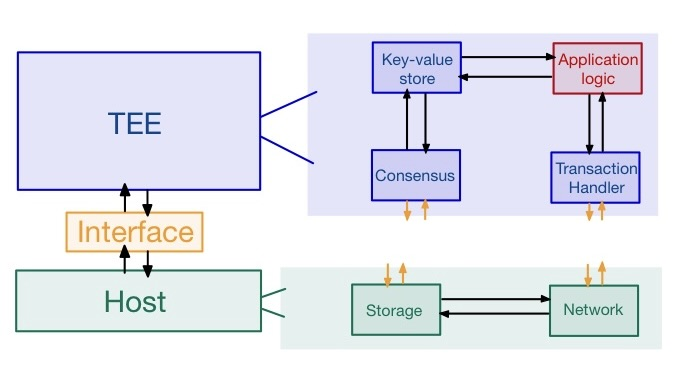
\includegraphics[scale=0.35]{pictures/basic_ccf}
	\caption{Each node consists of a TEE, the untrusted host, and an interface between the host and the TEE. The TEE consists of a Key-value store, the Consensus, the Transaction Handler and the specific Application logic.The storage and the network are placed outside the TEE.}
	\label{ccf}
\end{figure}
\subsection{Confidentiality}
\subsection{Reconfiguration}
Reconfiguration is the procedure when a node fails and is replaced by a new one. CCF therefore allows to add new or delete old nodes. Reconfiguration is implemented as a transaction.
\subsection{Desaster Protocol}
\subsection{TCB}
\subsection{Challenges}
As mentioned before CCF does not have a rollback detection, because it allows rollback attacks to happen, because it is not affecting the system. The problems are that they (1) make the assumption that the code inside the TEE cannot be changed and (2) that thy put their persistent storage outside the TEEs and is therefore not protected for a rollback attack.